%!TEX root = ../Thesis.tex
\chapter{structureOfSolubility}

The decision tree ensemble random forest have a series of useful diagnostics which have been used in this thesis work.

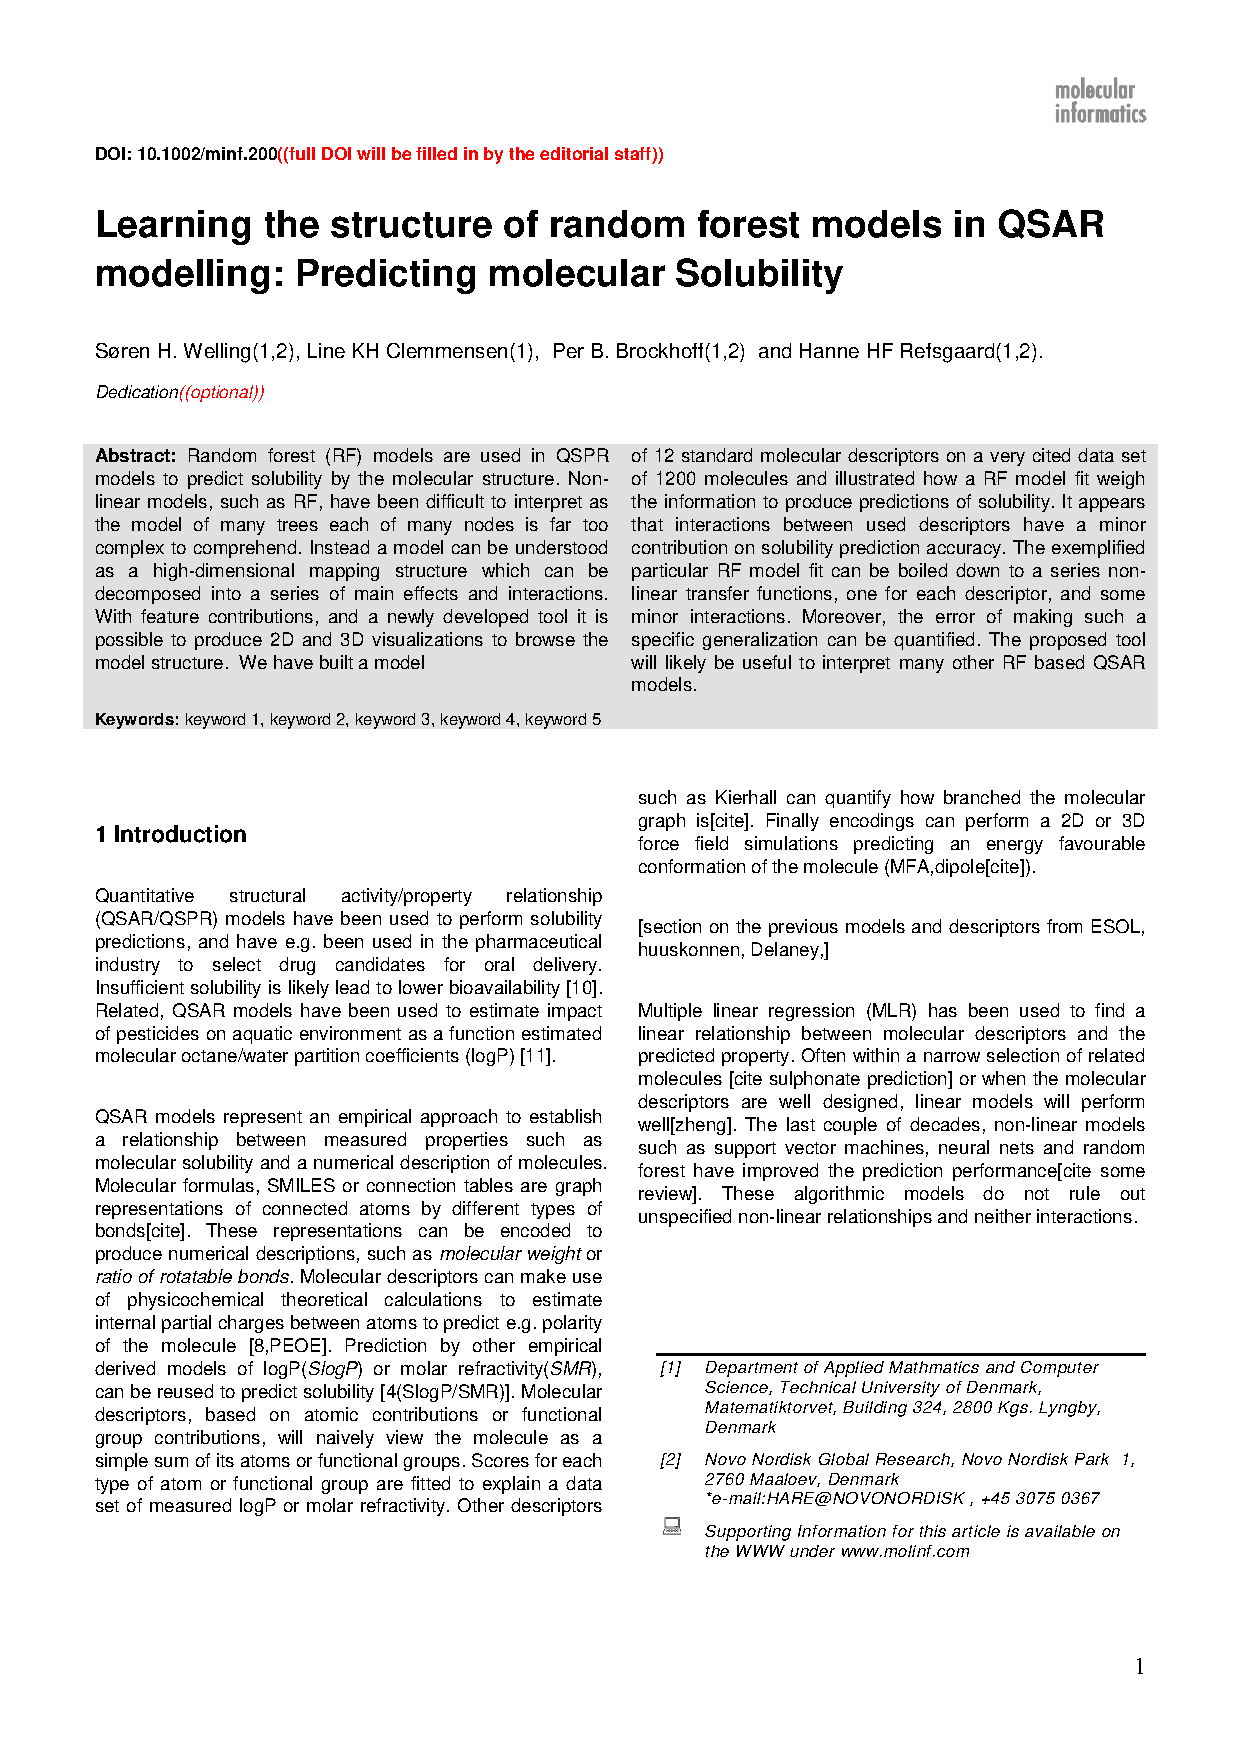
\includepdf[pages={1-},scale=0.90,pagecommand={\pagestyle{myruled}}]{chapters/structureOfSolubility.pdf}


\subsection{The correct temperature}
Solubility models (cite) are mainly derived from solubility measurements at room temperature 20-25 degrees Celcius. As the solubilization occurs at 37 degrees Celcius, some attractants may improve solubility more than others. A very new approach to predict solubility, at any temperature to first build a model predicting change of solubility as function of temperature. It is more difficult to acquire a data set with measured solubility at various temperatures than at room temperture only and the data set is like much smaller. Therefore a one approach is to model the temperature sensitivity for a smaller data set and use these temperature sensitivity predictions to a standard room temperature solubility prediction \cite{klimenko2016novel}.